\documentclass[twoside,english]{article}
%~ \usepackage{booktabs}
\usepackage{graphicx}
%~ \usepackage{subfigure}
%~ \usepackage{histogr}
%~ \usepackage{rotating}
\usepackage{amssymb,amsmath}

\newcommand{\union}{\mathrel{\cup}}
\newcommand{\unionprefix}{\mathopen{\cup}\ensuremath{\,}}
\newcommand{\intersection}{\mathrel{\cap}}
\newcommand{\intersectionprefix}{\mathopen{\cap}\ensuremath{\,}}
\renewcommand{\setminus}{\mathrel{\backslash}}
\newcommand{\powerset}{\mathopen{\mathbb{P}}\ensuremath{\,}}

\title{Key States}
\author{Yuri Schaeffer, Yuri@NLnetLabs.nl}
\date{\today}

\parindent 0pt
\parskip 5pt

\begin{document}
\maketitle{}

\tableofcontents

\section{Key State}

As Matthijs pointed out the state of a key can be described with individual
states for each component (DS, DNSKEY, RRSIG). Since these are all 
resource records I hope to use a common state diagram for all types.

TODO:
Regardless of the record type we can define 5 basic states. The 
distinctive property is its existence in caches world wide, so we 
choose a cache oriented approach. A record 
starts in a Generated state, $G$. Since the record is never 
published yet there is no cache having\footnote{When we say a record 
is in cache we explicitly mean that there are no old versions in 
cache with an unexpired TTL. Having to fetch a record from the 
authorities is also considered in cache.} this record. The next state is 
Submitted, $S$. In this state the record could be known to \emph
{any} cache, but might as well be none. As for all state the exact 
meaning depends on the record type, e.g. Submitted may mean emailed 
to parent or published in zone. State three is Propagated, $P$, 
which means all caches have the record or can obtain it. In the 
Withdrawn $W$ state not all caches have the record or are able to 
get it. Finally Ceased $C$ denotes no cache will try to use the 
record any longer.

To summarize:

\begin{description}
       \item[$G$] The record is not used.
       \item[$S$] Submitted, some caches might have seen the record.
       \item[$P$] Propagated, all caches have seen the record or will see it.
       \item[$W$] Withdrawn, some caches are unable to get the record.
       % \item[$C$] Ceased, the record is cashed nowhere.
\end{description} 

\section{State Transition}

Let $\mathbb{R}$ be the set of possible resource records, according to the
RFCs.  Note that this includes all possible records, including many
that make no sense to any zone owner anywhere.

% Yuri: \powerset(X) means the set of all subsets of X

Model a cache as the set of resource records from $\mathbb{R}$ that it currently
holds.  The type of the cache is $C:\powerset(\mathbb{R})$.  We will assume
that every cache adheres to the timing constraints imposed upon it by RFCs.
These constraints cannot be made explicit in this model, because this model
captures the (possible) situation(s) at a certain point in time.  A more
elaborate model, such as a Petri net, may add timing and thus capture the
additional detail.

\begin{figure}[t]
	\begin{tabular}{lll}
	$\emptyset$ & Empty set & $\emptyset = \{ \}$ \\
	$X\cup Y$ & Union between two sets & $\{1,2\} \cup \{2,3\} = \{1,2,3\}$ \\
	$X\cap Y$ & Intersection of two sets & $\{1,2\} \cap \{2,3\} = \{2\}$ \\
	$X\setminus Y$ & Set subtraction & $\{1,2\}\setminus \{2,3\} = \{1\}$ \\
	$\union X$ & Union iterated over set elements & $\union\{X,Y,Z\} = X\cup Y\cup Z$ \\
	$\intersection X$ & Intersection over set elements & $\intersection\{X,Y,Z\} = X\cap Y\cap Z$ \\
	$\powerset(X)$ & Powerset, or set of all subsets & $\powerset(\{1,2\}) = \{ \emptyset, \{1\}, \{2\}, \{1,2\}\}$ \\
	\end{tabular}
	\caption{Mathematical notation used}
\end{figure}

\paragraph{Caches.}
It is particularly useful to model a set $\mathbb{C}\subseteq\powerset(\mathbb{R})$ of all
possible caches around the World, as this represents all possible states
that could challenge a DNSSEC signer to behave properly.  Again, this
model will not capture the timing constraints that define precisely what
subset of $\powerset(\mathbb{R})$ actually forms $\mathbb{C}$.

% Yuri: Meestal gebruik je \mathbb alleen voor speciale (meta) gevallen

Based on these definitions, we can derive a meaningful partition of the
resource records $\mathbb{R}$ depending on how widely it is published:
%
\begin{eqnarray}\label{states}
	\emph{Hidden} &=& \mathbb{R}~\setminus~\unionprefix \mathbb{C} \\
	\emph{Propagating} &=& \unionprefix \mathbb{C}~\setminus~\intersectionprefix \mathbb{C} \\
	\emph{Omnipresent} &=& \intersectionprefix \mathbb{C}
\end{eqnarray}

\paragraph{Setting a goal.}
The above partition of $\mathbb{R}$ suffices to know what can be relied upon from the
caches in the World.  But, since DNS is not a static system, this state will evolve
with time.  Specifically, the \emph{Propagating} state is a temporary one that will be
departed as soon as the right TTL timing has passed.  This however, can go either
way; it depends on a new model element which way.  This model element is the goal
set for a resource record: Does it want to be \emph{Omnipresent} or \emph{Hidden}?

We therefore introduce another set named $\emph{Announced}\subseteq\mathbb{R}$ to hold
those resource records whose goal it is to end up in $\emph{Omnipresent}$.  Based on
this, it is possible to partition $\emph{Propagating}$ even further:
%
\begin{eqnarray}\label{states}
	\emph{Rumoured} &=& \emph{Propagating} \cap \emph{Announced}\\
	\emph{Squashed} &=& \emph{Propagating} \setminus \emph{Announced}
\end{eqnarray}

\begin{figure}[t]
	\centering
	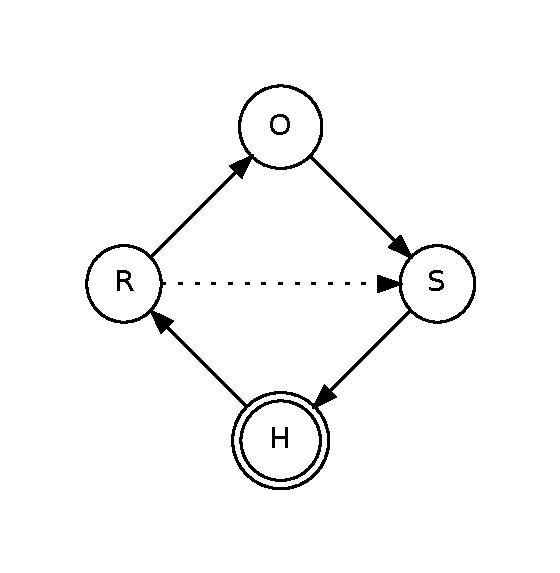
\includegraphics[scale=0.5]{states.pdf}
	\caption{State diagram for individual key components.}
	\label{fig:states}
\end{figure}

\paragraph{Predicate logic.}
The definitions above are in terms of set theory.  Although entirely equivalent, it is
probably useful to write the same thing in terms of predicate logic.  We introduce the
following boolean functions on $\mathbb{R}$, with shorthand names for reference in the
remaining pages of this document.

\begin{displaymath}
\begin{array}{lllll}
       H(r) & \equiv & r\in\emph{Hidden} &=& \forall c \in \mathbb{C}: r \not \in c \\
       R(r) & \equiv & r\in\emph{Rumoured} &=& (\exists c \in \mathbb{C}: r \not \in c) \wedge (\exists c \in \mathbb{C}: r\in c) \wedge r\in\emph{Announced}\\
       O(r) & \equiv & r\in\emph{Omnipresent} &=& \forall c \in \mathbb{C}: r \in c \\
       S(r) & \equiv & r\in\emph{Squashed} &=& (\exists c \in \mathbb{C}: r \not \in c) \wedge (\exists c \in \mathbb{C}: r \in c)\wedge r\notin\emph{Announced} \\
       %~ C(r) & \equiv & G(r)
\end{array}
\end{displaymath}



\subsection{Definitions}

Keys do not stand on their own, but actually require a number of resource records in
their context.  Specifically, a key and its context can be described as a tuple
$\langle\emph{ds},\emph{dnskey},emph{rrsig}\rangle$ with the resource records for
a DS, DNSKEY and RRSIG record, all for the same signing key.  Define the type
$K=\mathbb{R}\times\mathbb{R}\times\mathbb{R}$ represent such key with context.

\newcommand{\state}{\emph{State}}
\newcommand{\stateDS}{\emph{State}_\textrm{DS}}
\newcommand{\stateDNSKEY}{\emph{State}_\textrm{DNSKEY}}
\newcommand{\stateRRSIG}{\emph{State}_\textrm{RRSIG}}

Now define the following functions to capture the state $H$, $R$, $O$ or 
$S$
for each of the three components of a key with context tuple:
\begin{eqnarray*}
	\state(r) &\equiv& H\textrm{, if $r\in\emph{Hidden}$}\\
	          &\equiv& R\textrm{, if $r\in\emph{Rumoured}$}\\
	          &\equiv& O\textrm{, if $r\in\emph{Omnipresent}$}\\
	          &\equiv& S\textrm{, if $r\in\emph{Squashed}$}\\
	\stateDS(r,x,y) &\equiv& \state(r)\\
	\stateDNSKEY(x,r,y) &\equiv& \state(r)\\
	\stateRRSIG(x,y,r) &\equiv& \state(r)
\end{eqnarray*}

\begin{itemize}
	%~ \item $\mathbb{C}$ is a set of all caches
	%~ \item Cache $c \in \mathbb{C}$, a set of record sets r
	\item Key $k = \langle ds, dnskey, rrsig\rangle$, a tuple of states
	\item Key chain $\mathbb{K}$, a set of keys
	%~ \item $State(r) \in \{H, R, O, S\}$, with r one from k.
	\item $Goal(k) \in \{O, H\}$
	\item $Roles(k) \subseteq \{ksk, zsk\}$
	\item $Alg(k) \in \mathbb{N}$, Algorithm number of key
\end{itemize}

Each zone has its own key chain (but not necessarily unique key 
material). A key chain is a collection of keys currently involved with 
the zone, regardless of their state. The key itself consists of three 
states, one for each record involved. It also defines a goal to which
the records should try to move.

Each record is evaluated individually for the next state transition. 
If it not already reached its goal, it will try to move towards it 
provided the result is a valid DNSSEC configuration. This way only a 
small set of conditions is evaluated each time. 

Roll overs are not explicitly defined but derived from the 
set of rules. As a result the system or a user could insert a new key 
at any time in the process. For example a user has a dual key signing 
scheme and sets the goal of all current keys to Ceased. Then he inserts
a combined ZSK/KSK. From here the system will figure out the (save) way
to having the new key introduced. It might finish pending roll overs 
but if possible will try to discard the old keys as soon as possible.

Setting the goal of all your keys to ceased without first introducing 
a new key has no implication for the validity of the zone. The system 
always maintains a valid configuration. If it wants to remove old keys 
but can not, it won't.

%~ \subsection{Shorthands}
%~ 
%~ \begin{itemize}
	%~ \item This key is a KSK and active; we can rely on it. 
	%~ \\$kskready(k) \leftrightarrow ksk \in Roles(k) \wedge State(k_{ds}) = P \wedge State(k_{dnskey}) = P \wedge State(k_{rrsig}) = P$
	%~ \item If k' is a backup for k, k can safely be removed
	%~ \\$backupfor(k', k) \leftrightarrow k' \not = k \wedge Alg(k)=Alg(k') \wedge kskready(k')$
%~ \end{itemize}

\subsection{Transition rules for $Ds(k)$}

%~ \subsubsection{$State(k_{ds}) = H$}
\subsubsection{$H(Ds(k))$}
%~ \subsubsection{$H(State(Ds(k)))$}

\fbox{\begin{minipage}{\linewidth}

	%~ DS was never published so we can do a quick transition
	%~ \begin{equation}
		%~ \begin{split}
			%~ Goal(k)=C \rightarrow State(k_{ds})=C
		%~ \end{split}
	%~ \end{equation}

	If k is not a KSK the DS state does not matter. If is \emph{is}, before
	submitting either DNSKEY must be propagated or an other key with the 
	same algorithm should be ready.
	\begin{equation}
		\left.
		\begin{split}
			Goal(k)=O & \wedge ksk \not \in Roles(k) \\
			\\
			Goal(k)=O & \wedge O(Dnskey(k)) \\
			\\
			Goal(k)=O & \wedge 
				\exists k' \in \mathbb{K} 
				( \\
					& Alg(k)=Alg(k') \\
					& \wedge ksk \in Roles(k') \\
					& \wedge O(Ds(k')) \\
					& \wedge O(Dnskey(k')) \\
					& \wedge O(Rrsig(k')) 
				) 
		\end{split}
		\right\}\rightarrow [submit], R(Ds(k)) 
	\end{equation}
\end{minipage}}

\subsubsection{$R(Ds(k))$}

\fbox{\begin{minipage}{\linewidth}
	
	Nothing should depend on this RR yet.
	\begin{equation}
		\begin{split}
			Goal(k)=H \rightarrow S(Ds(k))
		\end{split}
	\end{equation}

	Has the user confirmed the DS is on its way to the parent and are 
	we sure everything propagated since then?
	\begin{equation}
		\left.
		\begin{split}
			Goal(k)=O & \wedge ksk \not \in Roles(k) \\
			\\
			Goal(k)=O 	& \wedge Confirmed(k_{ds}) \\
						& \wedge T_{now} \geq T_{whatever}
		\end{split}
		\right\}\rightarrow O(Ds(k))
	\end{equation}

	Postpone for later.

	\begin{equation}
		\begin{split}
			Goal(k)=O 	& \wedge Confirmed(k_{ds}) \\
						& \wedge T_{now} < T_{whatever} \\
						& \rightarrow [event]
		\end{split}
	\end{equation}
\end{minipage}}

\subsubsection{$O(Ds(k))$}

\fbox{\begin{minipage}{\linewidth}

	%~ A non-KSK can be set to withdrawn.
	%~ \begin{equation}
		%~ \begin{split}
			%~ Goal(k)=C \wedge ksk \not \in Roles(k) \rightarrow S(Ds(k))
		%~ \end{split}
	%~ \end{equation}

	DS may go in State W if it refers to nothing.
	Or if there are other keys with the same algorithm which are valid.
	Or we don't break other keys and we have some other valid key(s).
	\begin{equation}
		\left.
		\begin{split}
			Goal(k)=H 	& \wedge \forall r \in Roles(k) \\
			( \\
				& \exists k' \in \mathbb{K} ( k' \not = k \\
				&\wedge Alg(k) = Alg(k') \\
				& \wedge r \in Roles(k') \\
				& \wedge O(Ds(k')) \\
				& \wedge O(Dnskey(k')) \\
				& \wedge O(Rrsig(k'))) \\
			)\\
			\\
			%~ TODO: replace forall(implication) with not exists
			Goal(k)=H 	& \wedge ksk \in Roles(k) \\
			& \wedge \forall r \in Roles(k) \\
			( \\
				& \forall k' \in \mathbb{K} ( k' \not = k \\
					& \wedge Alg(k) = Alg(k')  \\
					& \wedge r \in Roles(k') \\ 
					& \rightarrow H(Ds(k'))
				)\\
				& \wedge \\
					&\exists k' \in \mathbb{K} (k' \not = k \\
					%~ & Alg(k) \not = Alg(k') \\
					& \wedge r \in Roles(k') \\
					& \wedge O(Ds(k')) \\
					& \wedge O(Dnskey(k')) \\
					& \wedge O(Rrsig(k'))
				) \\
			)\\
			\\
			Goal(k)=H 	& \wedge ksk \not \in Roles(k) \\
				& \wedge \exists k' \not \in \mathbb{K} (k' \not = k \\
				& Alg(k) = Alg(k') \\
				& \wedge ksk \in Roles(k') \\
				%~ & \wedge State(k'_{ds}) = P \\
				%~ & \wedge O(Dnskey(k')) \\
				& \wedge \neg H(Dnskey(k')) \\
				& \wedge O(Rrsig(k'))
				)
		\end{split}
		\right\} \rightarrow S(Ds(k)) \\
	\end{equation}
\end{minipage}}

\subsubsection{$S(Ds(k))$}

\fbox{\begin{minipage}{\linewidth}

	We must wait till at least $T_{whatever}$ before transition to State 
	Ceased. As a bonus, ZSKs may transition immediately.
	\begin{equation}
		\left.
		\begin{split}
			%~ Goal(k)=H & \wedge 
			ksk \not \in Roles(k)\\
			\\
			%~ Goal(k)=H 	& \wedge 
			T_{now} \geq T_{whatever}
		\end{split}
		\right\} \rightarrow H(Ds(k))
	\end{equation}

	\begin{equation}
		\begin{split}
			%~ Goal(k)=H 	& \wedge 
			T_{now} < T_{whatever}
						& \rightarrow [event]
		\end{split}
	\end{equation}
\end{minipage}}


\subsection{Transition rules for $k_{dnskey}$}

\subsubsection{$H(Dnskey(k))$}

\fbox{\begin{minipage}{\linewidth}

	%~ We want to move away from this key and DNSKEY was never published, retire immediately.
	%~ \begin{equation}
		%~ \begin{split}
			%~ Goal(k)=C \rightarrow State(k_{dnskey})=C
		%~ \end{split}
	%~ \end{equation}

	If the signatures are propagated we may submit the Dnskey. 
	Some other valid key is also acceptable.
	\begin{equation}
		\left.
		\begin{split}
			Goal(k)=O &\wedge O(Rrsig(k))\\
						&\wedge zsk \in Roles(k) \\
			\\
			Goal(k)=O & \wedge O(Rrsig(k))\\
					& \wedge \exists k' \in \mathbb{K}( \\
					& Alg(k')=Alg(k) \\
					&\wedge zsk \in Roles(k') \\
					&\wedge O(Ds(k')) \\
					&\wedge O(Dnskey(k')) \\
					&\wedge O(Rrsig(k'))) \\
			\\
			Goal(k) = O 
				&\wedge \forall r \in Roles(k) \\
				(\\
					& \exists k' \in \mathbb{K}(k' \not = k \\
					&\wedge Alg(k')=Alg(k) \\
					&\wedge r \in Roles(k') \\
					&\wedge O(Ds(k')) \\
					&\wedge O(Dnskey(k')) \\
					&\wedge O(Rrsig(k'))) \\
				)\\
		\end{split}
		\right\} \rightarrow R(Dnskey(k))
	\end{equation}
\end{minipage}}

\subsubsection{$R(Dnskey(k))$}

\fbox{\begin{minipage}{\linewidth}

	Skip the propagated state. Nobody heard of it anyway.
	\begin{equation}
		\begin{split}
			Goal(k)=H \rightarrow S(Dnskey(k))
		\end{split}
	\end{equation}

	We did wait long enough to make sure the dnskey record is known in 
	every cache?
	\begin{equation}
		\begin{split}
			Goal(k)=O \wedge T_{now} \geq T_{whatever} \rightarrow O(Dnskey(k))
		\end{split}
	\end{equation}

	We did not wait long enough: Wait some more.
	\begin{equation}
		\begin{split}
			Goal(k)=O \wedge T_{now} < T_{whatever} \rightarrow event(T_{whatever})
		\end{split}
	\end{equation}
\end{minipage}}

\subsubsection{$O(Dnskey(k))$}

\fbox{\begin{minipage}{\linewidth}

	If not part of a chain, withdraw. If there is still a DS make sure 
	there is some other valid chain for this algorithm. If none for 
	this algorithm are broken, some other algorithm will do as well.
	
	\begin{equation}
		\left.
		\begin{split}
			Goal(k)=H 
				&\wedge H(Ds(k))\\
				&\wedge H(Rrsig(k)) \\
			\\
			Goal(k)=H 
			%~ &\wedge State(k_{ds}) = C \\
				& \wedge \forall r \in Roles(k) \\
				(\\
				& \exists k' \in \mathbb{K} ( k' \not = k \\
				& \wedge Alg(k')=Alg(k) \\
				& \wedge r \in Roles(k') \\
				& \wedge O(Ds(k')) \\
				& \wedge O(Dnskey(k')) \\
				& \wedge O(Rrsig(k')) )\\
				) \\
				\\
			Goal(k)=H  &\wedge H(Ds(k))\\
				& \wedge \forall r \in Roles(k) \\
				(\\
				& \forall k' \in \mathbb{K} ( k' \not = k \\
				& \wedge Alg(k')=Alg(k) \\
				& \wedge r \in Roles(k') \\
				& \rightarrow H(Dnskey(k'))) \\
				& \wedge \\
				& \exists k' \in \mathbb{K} ( k' \not = k \\
				%~ & \wedge Alg(k') \not = Alg(k) \\
				& \wedge r \in Roles(k') \\
				& \wedge O(Ds(k')) \\
				& \wedge O(Dnskey(k')) \\
				& \wedge O(Rrsig(k')) )\\
				)
		\end{split}
		\right\} \rightarrow S(Dnskey(k))
	\end{equation}
\end{minipage}}

			%~ Goal(k)=C 	& \wedge State(k_{ds})=C \\
						%~ & \wedge State(k_{rrsig})=C \\
			%~ \\
			%~ Goal(k)=C 	& \wedge State(k_{ds})=C \\
						%~ & \wedge (\exists k' \in \mathbb{K}: k' \not = k \\
						%~ & \wedge Alg(k) = Alg(k')\\
						%~ & \wedge State(k'_{dnskey}) = P \\
						%~ & \wedge State(k'_{rrsig}) = P) \\
						%~ & \wedge Roles(k) \subseteq Roles(k') \\
			%~ \\
			%~ Goal(k)=C 	& \wedge (\exists k' \in \mathbb{K}: k' \not = k \\
						%~ & \wedge Alg(k) = Alg(k')\\
						%~ & \wedge State(k'_{dnskey}) = P \\
						%~ & \wedge State(k'_{rrsig}) = P) \\
						%~ & \wedge (\exists k' \in \mathbb{K}: k' \not = k \\
						%~ & \wedge Alg(k) = Alg(k')\\
						%~ & \wedge State(k'_{dsy}) = P \\
						%~ & \wedge State(k'_{dnskey}) = P) \\
						%~ & \wedge Roles(k) \subseteq Roles(k') \\


\subsubsection{$S(Dnskey(k))$}

\fbox{\begin{minipage}{\linewidth}

	State may transition to Ceased given enough time passed to propagate 
	change. 
	%~ Or when DS is already Ceased (only the DS is waiting this 
	%~ transition).
	\begin{equation}
		\left.
		\begin{split}
			%~ Goal(K) &=H \wedge 
			ksk \not \in Roles(k)\\
			\\
			%~ Goal(k)&=H \wedge 
			T_{now} \geq T_{whatever}
			%~ \\
			%~ Goal(k)&=C \wedge State(k_{ds})=C
		\end{split}
		\right\}\rightarrow H(Dnskey(k))
	\end{equation}

	Else, schedule event.
	\begin{equation}
		\begin{split}
			%~ Goal(k)=H \wedge 
			T_{now} < T_{whatever} \rightarrow event(T_{whatever})
		\end{split}
	\end{equation}
\end{minipage}}

\subsection{Transition rules for $k_{rrsig}$}

\subsubsection{$H(Rrsig(k))$}

\fbox{\begin{minipage}{\linewidth}

	%~ Nobody ever saw this signatures, we won't need it.
	%~ \begin{equation}
		%~ \begin{split}
			%~ Goal(k)=C
		%~ \end{split}
		%~ \rightarrow State(k_{rrsig})=C
	%~ \end{equation}

	Signatures for ZSKs can be introduced. For KSKs there must be a 
	valid ZSK.
	\begin{equation}
		%~ \left.
		\begin{split}
			Goal(k)=O 
		\end{split}
		%~ \right\} 
		\rightarrow R(Rrsig(k))
	\end{equation}
\end{minipage}}

\subsubsection{$R(Rrsig(k))$}

\fbox{\begin{minipage}{\linewidth}

Don't wait till signatures are propagated.
	\begin{equation}
		\begin{split}
			Goal(k)=H \rightarrow S(Rrsig(k))
		\end{split}
	\end{equation}

Enough time passed to propagate signatures. Or if we do a smooth 
transition 
	\begin{equation}
		\left.
		\begin{split}
			Goal(k)=O &\wedge T_{now} \geq T_{whatever} \\
			\\
			Goal(k)=O & \wedge AllowSmooth \\
					& \wedge \forall r \in Roles(k) (\\
						& \exists k' \in \mathbb{K} ( \\
							& Alg(k') = Alg(k) \\
							& \wedge r \in Roles(k') \\
							& \wedge O(Dnskey(k')) \\
							& \wedge O(Rrsig(k')) \\
						)
					)
		\end{split}
		 \right\} \rightarrow O(Rrsig(k))
	\end{equation}
	


Not enough time passed to propagate signatures.
	\begin{equation}
		\begin{split}
			Goal(k)=O \wedge T_{now} < T_{whatever} \rightarrow event(T_{whatever})
		\end{split}
	\end{equation}
\end{minipage}}


\subsubsection{$O(Rrsig(k))$}

\fbox{\begin{minipage}{\linewidth}

	If the dnskey is gone from all caches can we withdraw the 
	signatures. We may break the chain if other valid keys are 
	available.

	\begin{equation}
		\left.
		\begin{split}
			Goal(k)=H &\wedge H(Dnskey(k)) \\
			\\
			Goal(k)=H
				& \wedge \forall r \in Roles(k) \\
				( \\
				& \exists k' \in \mathbb{K} ( k' \not = k \\
					& \wedge Alg(k) = Alg(k') \\
					& \wedge r \in Roles(k')\\
					& \wedge O(Ds(k')) \\
					& \wedge O(Dnskey(k')) \\
					& \wedge O(Rrsig(k'))) \\
				)
		\end{split}
		\right\} \rightarrow S(Rrsig(k))
	\end{equation}
\end{minipage}}

\subsubsection{$S(Rrsig(k))$}

\fbox{\begin{minipage}{\linewidth}

	Dnskey is gone so no one needs these signatures.
	\begin{equation}
		\left.
		\begin{split}
			%~ Goal(k)=H &\wedge 
			H(Dnskey(k)) \\
			\\
			%~ Goal(k)=H &\wedge 
			T_{now} \geq T_{whatever} 
		\end{split}
		\right\} \rightarrow H(Rrsig(k))
	\end{equation}

	\begin{equation}
		\begin{split}
			%~ Goal(k)=H \wedge 
			T_{now} < T_{whatever} \rightarrow event(T_{whatever})
		\end{split}
	\end{equation}
\end{minipage}}


\end{document}
